\chapter{Principios físicos}

El objetivo de esta clase es familiarizarze con los conceptos de combinación de bandas y firma espectral, utilizando nuevamente el software SNAP. Se realizarán diferentes combinaciones de bandas teniendo en cuenta la respuesta de los usos y coberturas en función de la combinación de colores. 





\section{Combinación de bandas}
En esta ocasión vamos a realizar diferentes combinaciones de bandas analizando en la visualización, la variación de los diferentes usos y coberturas del suelo y la vegetación en la imagen/escena.

%desarrollar un poco

\subsection{Combinación color real}\label{sec:colorreal}

Abra la imagen \begin{center} \directory{S2B\_MSIL2A\_2018-01-31.dim}.
\end{center} seleccione \menu{Open RGB image windows} haciendo click derecho sobre el nombre de la imagen. Se desplegará una nueva ventana (Figura \ref{fig:RGB}) que le permitirá elegir la combinación de bandas. Por defecto aparecerá la combinación color real que utiliza las bandas \emph{rojo (B4)}, \emph{verde(B3)} y \emph{azul(B2)} de \emph{Sentinel-2}. Desplieguela haciendo click en \menu{OK}.

En esta combinación, las características del suelo aparecen en colores similares a su apariencia para el sistema visual humano. Es así que la vegetación sana se observa en tonalidades de verde, los suelos recientemente cosechados o compactados se observan brillantes, en tanto que la vegetación senescente o de escasa cobertura se observa en tonos de marrón y amarillo. Por otro lado, esta combinación de bandas presenta mayor respuesta a cuerpos de agua, resaltando características como sedimentos, profundidad o presencia de floraciones algales.

Utilice el mapa con puntos de interés para identificar y familiarizarse con los diferentes usos y coberturas (Figura \ref{fig:mapa}). Explore la ubicación de los puntos mencionados utilizando las herramientas de navegación y zoom  (Figura \ref{fig:mono}). Compare color, tono y textura para cada punto.


\subsection{Combinación infrarrojo color}
\label{sec:infrarrojocolor}

Seleccione \menu{Open RGB image windows} haciendo click derecho sobre el nombre de la imagen. Se desplegará una nueva ventana (Figura \ref{fig:RGB}) que le permitirá elegir la combinación de bandas. Seleccione las bandas \emph{infrarrojo cercano (B8)}, \emph{verde(B3)} y \emph{azul(B2)} de \emph{Sentinel-2}. Desplieguela haciendo click en \menu{OK}.

En esta combinación, la vegetación aparece en tonos de rojo y magenta, las áreas urbanas se pueden observar en tonos de cian y los suelos varían en tonos de verde. El agua, por su parte, varía en tonos de azul. La vegetación leñosa (bosques) puede observarse en tonos rojizos en tanto que la vegetación herbácea (pastizales y cultivos) puede observarse en magenta. Esta combinación es útil para estudios de vegetación ya que resalta la relación entre el infrarrojo cercano y el rojo. Las áreas urbanas densamente pobladas se muestran en azul claro.

Utilice el mapa con puntos de interés para identificar diferentes tipos de vegetación (Figura \ref{fig:mapa}). Explore la ubicación de los puntos mencionados utilizando las herramientas de navegación y zoom  (Figura \ref{fig:mono}). Compare color, tono y textura para cada punto.

\subsection{Combinación vegetación sana}
\label{sec:vegetacionsana}

Seleccione \menu{Open RGB image windows} haciendo click derecho sobre el nombre de la imagen. Se desplegará una nueva ventana (Figura \ref{fig:RGB}) que le permitirá elegir la combinación de bandas. Seleccione las bandas \emph{infrarrojo cercano (B8)}, \emph{infrarrojo onda corta(B11)} y \emph{azul(B2)} de \emph{Sentinel-2}. Desplieguela haciendo click en \menu{OK}.

La vegetación saludable aparece en tonos de rojos, marrones, naranjas y amarillos. Los suelos pueden estar en verdes y marrones, las áreas urbanas pueden observarse en blanco y cian, las áreas de color azul intenso representan suelos sin cobertura vegetal y las áreas color rosa muestran vegetación en crecimiento . El agua clara y profunda se observa oscura; si el agua es poco profunda o contiene sedimentos, aparecería como tonos de azul más claro. Para estudios de vegetación, la adición de la banda del infrarrojo de onda corta aumenta la sensibilidad para identificar estrés hídrico y variaciones en el contenido de humedad en la vegetación y suelos.

Utilice el mapa con puntos de interés para identificar diferentes tipos de vegetación (Figura \ref{fig:mapa}). Explore la ubicación de los puntos mencionados utilizando las herramientas de navegación y zoom  (Figura \ref{fig:mono}). Compare color, tono y textura para cada punto.

\section{Firmas espectrales}


En esta ocasión vamos a analizar el comportamiento espectral de diferentes usos y coberturas.

\section{Seleccion de imagen}

Seleccione la combinación "vegetación sana" \emph{infrarrojo cercano (B8)}, \emph{infrarrojo onda corta(B11)} y \emph{azul(B2)} de \emph{Sentinel-2} y visualicela utilizando una sola ventana de la vista. Para ello vaya a \menu{Window} y seleccione \menu{Tile Single}

\begin{figure}[h!]
    \centering
    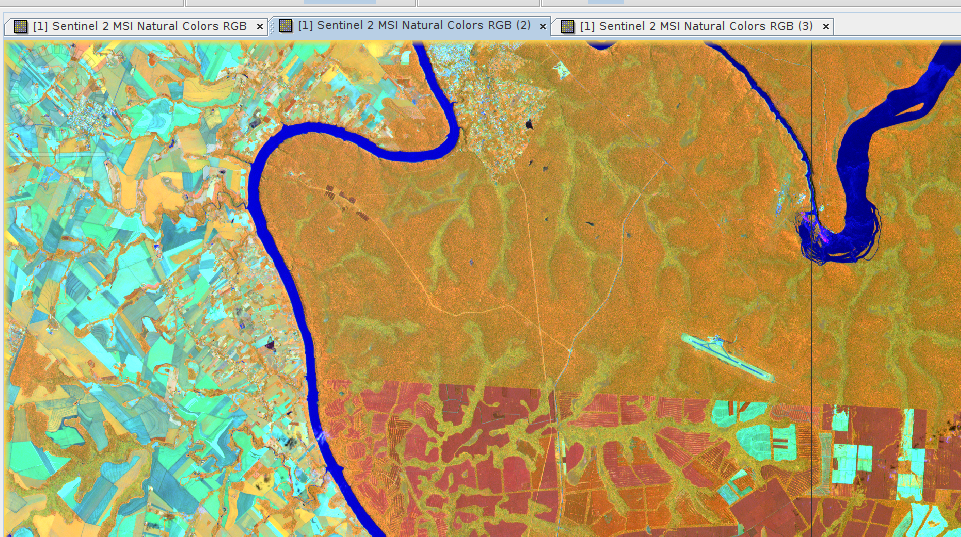
\includegraphics[width=0.6\textwidth]{fig:multiple-single.png}
    \caption{Distintas imágenes desplegadas en multiples visualizadores en simultaneo.}
    \label{fig:multiples}
\end{figure}

\section{Utilización de puntos}

El siguiente paso será seleccionar puntos de interés en los cuales evaluaremos el comportamiento espectral de diferentes usos y coberturas del suelo. A tal fin utilizaremos la herramienta \menu{pin placing tool} para tomar puntos de muestreo para firmas espectrales.

\begin{figure}[h!]
    \centering
    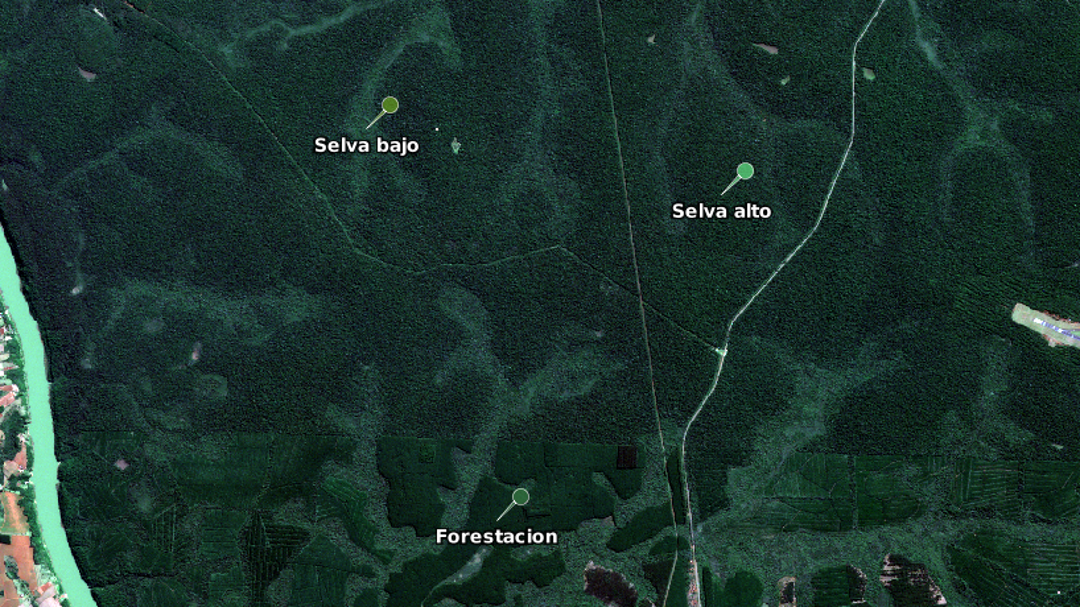
\includegraphics[width=0.05\textwidth]{fig:pin.png}
    \caption{Herramienta pin placing tool.}
    \label{fig:pin}
\end{figure}

Identifique en el mapa (Figura \ref{fig:mapa}) un parche homogéneo de selva paranense y añada un pin con la herramienta \menu{pin placing tool}:

\begin{figure}[h!]
    \centering
    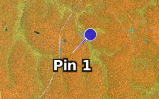
\includegraphics[width=0.2\textwidth]{fig:pin-selva.png}
    \caption{Pin en un parche homogéneo de selva paranaense.}
    \label{fig:selva}
\end{figure}

Para cambiar del Pin características como nombre o color ir a \menu{View>Tool Windows>Pin Manager}. Seleccionar en la columna \menu{label} el nombre Pin 1 y cambiar por "selva paranaense". En la columna \menu{color} asignar el color deseado.

\section{Visualización de firmas espectrales}

Ahora procederemos a visualizar la firma espectral correspondiente al Pin creado. Seleccione \menu{Optical>Spectrum View}. Se desplegará el visor de firmas espectrales. Para visualizar el Pin creado, seleccione la herramienta \menu{Show spectra for all pins}


Ahora procederemos a identificar y comparar firmas espectrales de diferentes usos y coberturas. Con la ayuda del mapa (Figura \ref{fig:mapa}) identifique parches homogéneos de bosque implantado, cultivo, suelo sin cobertura vegetal y cuerpo de agua e inserte en cada uno de ellos un pin con la herramienta \menu{pin placing tool}. A medida que vaya generando cada pin, recuerde modificarle las caracteristicas con la herramienta  \menu{View>Tool Windows>Pin Manager}. A continuación visualice las firmas correspondientes a los pins generados utilizando la herramienta \menu{Optical>Spectrum View}.

\begin{figure}[h!]
    \centering
    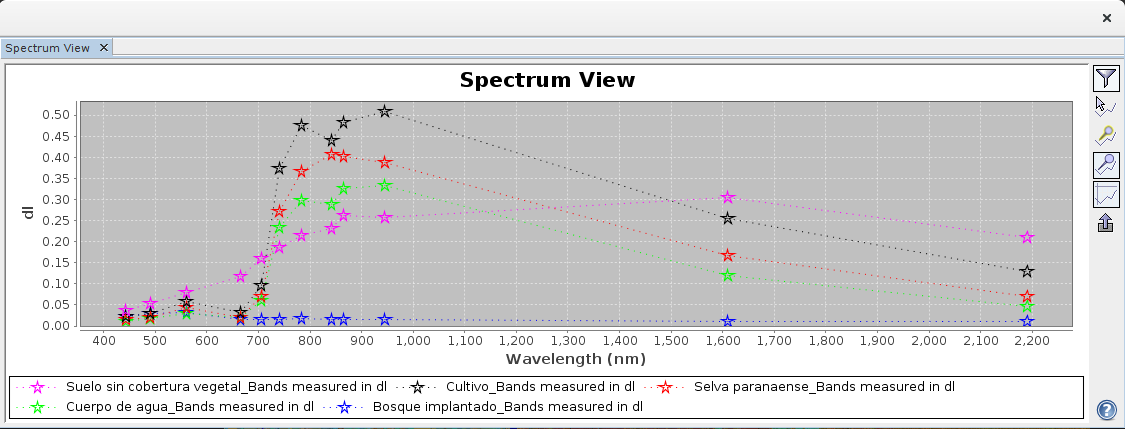
\includegraphics[width=0.7\textwidth]{fig:spectral-signature.png}
    \caption{Ejemplo de firmas espectrales obtenidas}
    \label{fig:spectral-signature}
\end{figure}

\section{Actividad práctica}
\begin{enumerate}
  \item Despliegue las tres combinaciones realizadas utilizando múltiples visualizadores(Figura \ref{fig:mono}). Utilice las herramientas \menu{Panning tool} y \menu{Zooming tool} e identifique la intersección del río Paraná y río Iguazú (Figura\ref{fig:mapa} punto de referencia 4):
  \begin{enumerate}
  \item Compare color y tono de los ríos Paraná e Iguazú. En base a interpretación visual ¿Que combinación considera la más adecuada para identificar sedimentos? ¿Cuál  considera que tiene mayor concentración de sedimentos?
  \item  Desplácese hasta Puerto Iguazú (\ref{fig:mapa} punto de referencia 11) y analice el área urbana. ¿En qué combinación puede ver con mayor nitidez la red víal?
  \item  Identifique el embalse Urugua-í (\ref{fig:mapa} punto de referencia 6) y compare la presencia de sedimentos con los ríos Paraná y Iguazú. ¿Cuál de ellos presenta menor concentración de sedimentos?
\end{enumerate}

  \item Identifique en el mapa de referencia los puntos 1 y 4 correspondientes a Selva Paranaense y Bosque Implantado respectivamente (Figura\ref{fig:mapa}) y compare:
  \begin{enumerate}
    \item  Compare color y tono de la selva paranaense y el bosque implantado para color natural.
    \item  Compare color y tono de la selva paranaense y el bosque implantado para infrarrojo color.
    \item  Compare color y tono de la selva paranaense y el bosque implantado para la combinación "vegetación sana".
    \item Compare ahora ambas coberturas con los tres visualizadores. ¿En qué combinación encuentra mayor heterogeneidad? ¿Cuál considera que es la más útil para separar diferentes tipos de vegetación?
    \item Compare un cultivo con cobertura vegetal contra un lote de suelo sin cobertura (\ref{fig:mapa} punto de referencia 8 y 9) ¿Qué combinación considera más útil para medir heterogeneidad para suelo sin cobertura vegetal? ¿y para suelos con vegetación?
  \end{enumerate}

  \item Seleccione entre las pestañas abiertas la que corresponda a la combinación color real (Sección \ref{sec:colorreal}). Inserte un pin para el río Paraná, río Iguazú y embalse Urugua-í. Modifique el nombre y color de los mismos con la herramienta \menu{Pin Manager} y grafique con la herramienta \menu{Spectrum View}
  \begin{enumerate}
      \item Compare las tres firmas espectrales. Analice el patrón de reflectancia. ¿Presentan todas el mismo patrón?
      \item Identifique picos y valles de reflectancia. ¿Que cuerpo de agua presenta mayor reflectancia en el visible-NIR? ¿Cuál presenta menor? Analice los factores biofísicos que modelan este comportamiento.
    \end{enumerate}

  \item Seleccione entre las pestañas abiertas la que corresponda a la combinación vegetación sana (Sección \ref{sec:vegetacionsana}). Inserte un pin para selva paranaense, bosque implantado, cultivo y suelo sin cobertura vegetal. Modifique el nombre y color de los mismos con la herramienta \menu{Pin Manager} y grafique con la herramienta \menu{Spectrum View}
  \begin{enumerate}
    \item Analice las cuatro firmas espectrales teniendo en cuenta los picos y valles de reflectancia de acuerdo a la longitud de onda correspondiente. ¿En qué longitudes de onda presenta mayor reflectancia la vegetación? ¿En cuáles presenta menor reflectancia? Analice teniendo en cuenta los parámetros fisiológicos que modelan este comportamiento.
    \item Compare una firma de vegetación fotosintéticamente activa (e.g. selva paranaense) con otra de suelo sin cobertura vegetal. ¿Muestra una separación en el visible? ¿Y en el infrarrojo cercano? Analice donde se observan mayores diferencias.
  \end{enumerate}
	\item Identifique un área urbana, añada un pin. Modifique nombre y color. Compare con el resto de las firmas espectrales. ¿Que diferencias observa con respecto a suelo sin cobertura vegetal? ¿En qué regiones del espectro las observa?
  \end{enumerate}

Estas preguntas y actividades no serán evaluadas. Su objetivo es discutirlas en el foro de consultas e intercambio de la clase.

%Ver cómo manejar el tema de borrar pines en las comparaciones
% Añadir al anexo las longitudes de onda x mision satelital.
